\section{Introduction}

\subsection{Driving Support Systems}

In this document we are mainly concerned about driving assistance. However, driving assistance is a vast research field with almost a century of evolution. Such systems aims to support the driver in the action of driving, this support is given in any form: visual alerts, auditory perception, actuators or haptics\cite{riener2010sensor}.

Since its appearance at the middle 50's, driving assistance has gained several branches, those branches have been heavily studied and currently are the target of many research centers.

Drive-support systems are becoming more and more popular. There exist several reasons, all of them mostly related with reducing \textbf{risk of incidents} and/or increasing the \textbf{confort} of driving. 

The former is linked with the cognitive overload in which the human is submited to. Off course the cognitive limitation is not an absolute number, it varies according to several parameters like mental health, type of the channel used (visual, auditory, tactile), amount of information transmitted, etc. A research conducted 2008 had the intend to study the human cognitive limitation for visual (eye) channel, basing this limitation in the saccadic movement of the eye and in the channel information capacity theorem\cite{LautarutisV}. The latter is linked to the anatomy of the instruments and the means used by the driver to perform an activity.

The human eye provides the largest amount of information for the brain. As the human visual sensors gives the major part of the world perception to the brain, it becomes per consequence the most used sensor.

The action of driving did not change since its creation, but the environment has. Due to this evolution the Advanced Driver Assistence Systems (ADAS) was coined to characterize advanced techniques that enhances the capability of driving, improving the vehicle-handling performance and at the same time reduce the workload for the driver\cite{riener2010sensor}.

The engineering of those types of systems is not related directly to computer science. The first mechanisms ever created for driving-support were purely mechanic, some examples of such systems are Cruise Control(CC), Anti-lock Break System (ABS), Collision Avoidance System(CAS).

Advanced Driver Assistence Systems must to perceive the environment before act. ADAS, just like the human cognition, requires a mean to perceive the environment before dispatch any cognitive action. In the humanbody this is addressed for the human eyes, but ADAS requires some other kind of sensing, sense that mimics the environment perception just like the human eyes. 

The different ways of perceiving the environment and different types of technology used to achieve characterizes the sensing instruments, usually called \textbf{sensors}.

%% reviewed until here

For decades academics researchers have studying and trying to understand and mimic the human vision perception in the robotics field, as the vision is a ground bases for human condition, this has a trivial meaning through a human perspective, but mimic this characteristics is extremely complex.

Starting from vision, there exists several approaches and technologies that provide a representation of the environment: Radio frequency(RADAR), Electromagnet radiation (generally an invisible wave length), photograph representation. Those methods differentiate in the cost of equipment and the treatment in which their output must go through so the information can be used as an input.

The goal of having those representations, depending on the requirements of the application, is to track the objects, perform classification, data association, etc.

In this paper we are concerned with electromagnetic radiation scanners, LIDAR(Light Detection and Ranging) laser for instance.

The LIDAR laser scanners output is the basis for development of this work. As input of our algorithm we use Bayesian Occupancy Filter \cite{TAY-2008-295084} to cope with the uncertainty of the information given by the sensor measurements. As a rule of thumb the measurements require an estimation framework to correct, or least, approximate the measurements from the real data.

As our test platform is a vehicle, this kind of sensor is embedded in a vehicle as a set of sensors with different layers.

By the end of this report, we will present the results achieved and the uncertainty generated by the sensor measurements and its impacts in algorithm outputs.

%\end{comment}

\subsection{Sensors}



\subsection{Spatial representation}

There exists several ways to represent one environment in with respect to its spatial information. Occupancy Grid is one of these methods and it is largely applied, its built based on a multidimensional field that maintains the occupancy state information in a cell\cite{Elfes:1989:UOG:68491.68495}. Those cells are built in a regular size, and the number of cells which compose the grid is algorithm dependent. 

At the same time Occupancy Grid (a.k.a. certainty grids) is effective in data representation it is also effective in represent sensor fusion information with it. Occupancy grid can be used as well to represent tree-dimentional environment, as was demonstrated in a small submersible craft, that looks for old battleships in the bottom of the ocean\cite{DBLP:journals/aim/Moravec88}.

One variation of the occupancy filter - The Bayesian Occupancy Filter(BOF) - contains the velocity and the probability distribution in Bayesian framework.


\subsubsection{SLAM}

SLAM (Simultaneous Localization and Mapping) is a concurrent map and localization problem, where the initial position of the ego-robot is unknown. The SLAM uses the observation done by the robot's sensor to localize the ego-robot in the environment and build the map at the same time\cite{VU-2009-454238}. 

But in this model it's required that we have a precise map - by precise we mean an exact map, exact enough for be considered as unreal and not achievable. This precision is required duo to simultaneously as the robot move we must localize it in the map, and as the robot motion is performed in a continuous space, any interference in the measurements are accumulated and can affect severely the localization.

The robot motion depends on the contact surface, inertial forces, the type of the ground surface in which the robot should move, its weight, speed, etc.

All those variations bring an imprecision factor into the movement performed by a robot.

From the probabilist point of view, this implies in estimate the joint probability distribution (Equation \ref{jpd:discrete}). Where the $u$ represents the observations and $z$ the measurements.

Thus, the output of the SLAM process is the robot pose and a map of the stationary objects captured by the \textit{perception} sensors \cite{iyengar1991autonomous}.

%\begin{equation}
%\label{jpd:continuous}
%\int_a^b f(x) \, \mathrm dx
%\end{equation}

\begin{equation}
\label{jpd:discrete}
P(x_t,M | z_{0:t}, u_{1:t})
\end{equation}


\subsubsection{DATMO}

Detection and Tracking of Moving Objects was initially studied by radar tracking systems \cite{VU-2009-454238} researches. Thus, they capture only moving object in the instrument, with those objects in scene they must solve the data association problem. The former assumption is unrealistic in the vision of a robot, the perception sensor senses all objects, independently on their motion, so static and dynamic objects are included.

As DATMO is a large process, some researchers chose to pick just a part of this process, which is "Moving Object Tracking" and solve it, without worry about the detection phase.

\subsubsection{SLAMMOT}

Researches considered SLAM and DATMO as two different problems that should be solved separately, \textit{Wang} was one of the first researches to put in evidence the similarities between both problems \cite{Wang03onlinesimultaneous}.

As result, the SLAMMOT term was coined and a derivation of the SLAM formula with DATMO was created to simplify the process of tracking. The experiment showed that solving the SLAM with DATMO increased dramatically the performance of the algorithm comparing them with the results as individual solutions (performance was verified in crowded urban environment).

As the GPS system or an good IMU for a good precision are too expensive, the paper propose a bayesian approach solution which satisties the navigation constraints without compromise the safety and at the sametime are not high costly as the other solutions based on a specialized hardware.

\subsubsection{SLAM and DATMO}

Robots face a set of problems which are common among many robots, how to move in a certain environment is one of them.

The general environment perception (Figure \ref{fig:perception:cycle}) requires at least two inputs: the perception measurements $Z$ which are usually are provided by cameras, LIDAR, or even radars, and motion measurements provided by the IMU (Inertial Measurement Unit).

\begin{figure}[H]
   \centering
     \begin{tabular}{lr}
       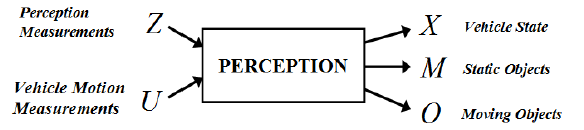
\includegraphics[scale=0.5]{img/fig:perception:cycle}
     \end{tabular}
   \caption{define}
   \label{fig:perception:cycle}
 \end{figure}


He perceives the environment by using as input sensors informations and can be composed of several sensors, or even heterogeneous types of sensors, and those give a partial observation of the environment (according with the current technology applied in those sensors). Thus, the robot does not known what paths can be perceived to reach a given point in a space.

So, knowing the positions that can be assumed by the robot is essential and necessary so robot cat move in this environment, this is done by observing the environment through the sensors and creating a spatial relation between the static objects in this space, this is known as SLAM - or Simultaneous Localizations and Mapping \cite{iyengar1991autonomous}.

Although, this just concern a small set of the problems related with robots applications, for instance robots that are used for mining, in this type of environment the only element that can change the environment and the spatial relation between the static objects is the robot itself. 

Depending in the goal of the robots perception, may be required to make distinction between each object, with cameras we can use characteristics like color, shape. Whereas, classify an object based in a LIDAR or radar information neither shape nor color are available, at least not directly without pre-processing.

Another set of problems concerns the most part of robots applications are highly dynamic environments, where the objects can change their position with respect to the static environment, those objects can become an obstacle for the robots, for this reason its necessary to map those objects, this relation called DATMO - Detection and Tracking of Moving Objects.

Although these two classification are given in a separate manner, they can be used as complementary to each other as presented in the paper \cite{Wang04a}, which will be dissected later.

\subsection{Occupancy grid mapping}

Representing continous space when dealing with the uncertainty of an action of a mobile robot is extremely demanding in terms of resource usage, either in terms of processing power or memory allocation.

Thus, targeting to amortize the computational requirement for the incertainty in the displacement of a robot, discretization models are used, Occupancy Grid\cite{Elfes:1989:UOG:68491.68495} is one of the former models proposed to tackle this issue.

This kind of representations is done with multi-dimensional vectors and results in a bird-eye view of the discretized map obtained by the perception sensor Figure \ref{fig:grid:continuous:discretized}.


\begin{figure}[H]
\centering
	\begin{tabular}{lr}\\
		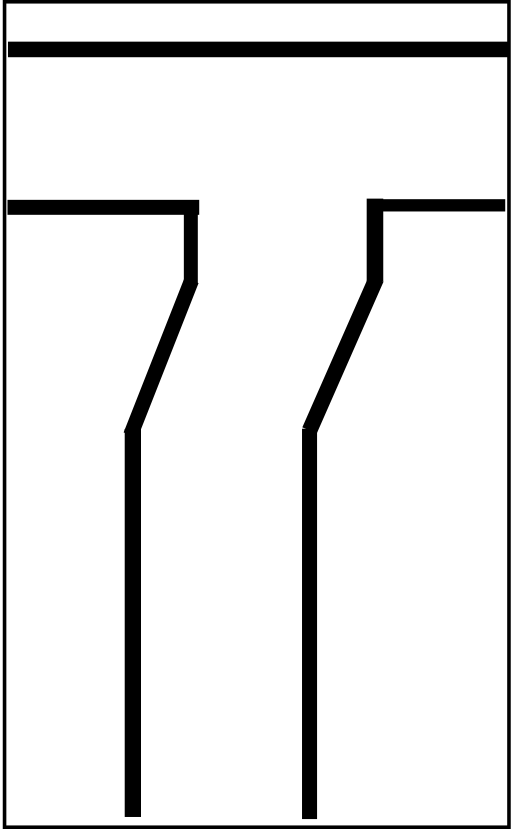
\includegraphics[width=0.25\columnwidth]{img/fig:grid:continuous} &
		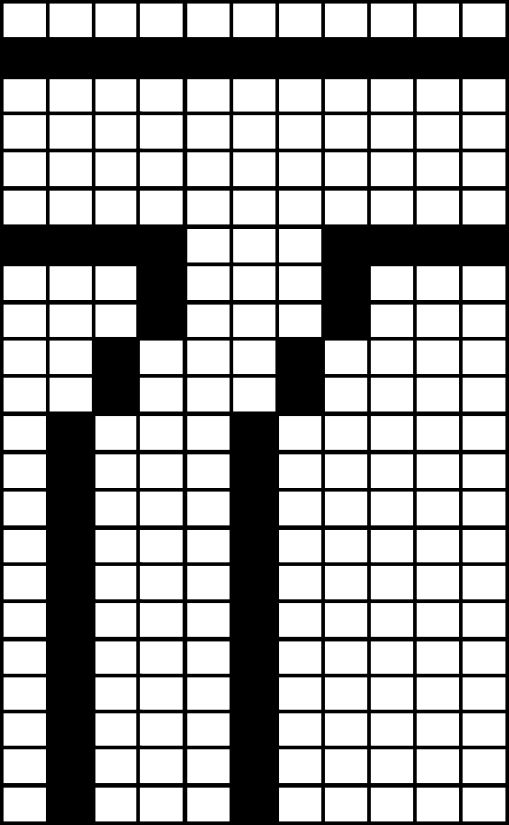
\includegraphics[width=0.25\columnwidth]{img/fig:grid:discretized}
	\end{tabular}
	\caption{Continuous \& discretized representation of a map}
	\label{fig:grid:continuous:discretized}
\end{figure}


In grid framework each cell $C$ can be assigned have its state $\phi(C)$ configured to binary domain, so, either the current state of the cell is \textit{occupied} or it is \textit{free}, in this paper we state that the value $1$ represents the occupied state and $0$ a $free$ space Equation \ref{eq:binarycell}.

\begin{equation}
P(\phi(C)=1) + P(\phi(C)=0) = 1
\label{eq:binarycell}
\end{equation}

This model can be extended to a more general model coined as \textit{inference grids} that encapsulate multiple properties\cite{Elfes:1989:OGP:916528}.

\textit{Goal: Why occupancy grid? how its built? }

\subsection{Object Separation}

\textit{Goal: u-disparity, uv-disparity}

\paragraph*{UV-disparity} 

UV disparity come off from an technique called U-disparity, a technique which aimed to separate the objects from the road surface.. (uv disparity slide 2)


\subsection{Classification}

\textit{Goal: talk about multimodels, importance sampling (or other statistical sampling method), prior map knowledge }

%multimodels, importance sampling, prior map knowledge
